\documentclass[12pt]{article}

% General
\usepackage[round]{natbib}
\usepackage{setspace}
\usepackage{geometry}
\usepackage[section]{placeins}
\usepackage[hidelinks]{hyperref}
\usepackage{graphicx}
\usepackage{xcolor}
\usepackage{titlesec}
\usepackage[page]{appendix}
\usepackage{enumerate}

% Tables/Figures
\usepackage{lscape}
\usepackage{booktabs}
\usepackage{rotating}
\usepackage{multirow}
\usepackage{longtable}
\usepackage{caption}
\usepackage{subcaption}
\usepackage{float}

% Math
\usepackage{amsmath}
\usepackage{amssymb}
\usepackage{amsthm}
\usepackage{mathtools}
\usepackage{dsfont}

\usepackage{tikz}

% \doublespacing
\onehalfspacing
% \singlespacing

% \numberwithin{equation}{section}

\geometry{paper=letterpaper, margin=1in}
\captionsetup{font=small}

% Code
\usepackage{textcomp}
\usepackage{sourcecodepro}
\usepackage{listings}
\definecolor{commentgrey}{gray}{0.45}
\definecolor{backgray}{gray}{0.96}
\lstset{
  basicstyle=\footnotesize\ttfamily, keywordstyle=\footnotesize,
  backgroundcolor=\color{backgray}, commentstyle=\color{commentgrey},
  frame=single, rulecolor=\color{backgray}, showstringspaces=false,
  breakatwhitespace=true, breaklines=true, upquote=true,
  numbers=left, numberstyle=\footnotesize\color{commentgrey}}

%%%%%%%%%%%%%%%%%%%%%%%%%%%%%%%%%%%%%%%%%%%%%%%%%%%%%%%%%%%%%%%%%%%%%%%%%%%%%%
% User-defined LaTeX commands
\DeclareMathOperator{\Var}{Var}
\DeclareMathOperator{\Cov}{Cov}
\DeclareMathOperator{\Corr}{Corr}
\DeclareMathOperator*{\argmax}{arg\,max}
\DeclareMathOperator*{\argmin}{arg\,min}
\DeclarePairedDelimiter{\abs}{\lvert}{\rvert}
\DeclarePairedDelimiter{\norm}{\lVert}{\rVert}
\newcommand*{\expp}[1]{\exp\left(#1\right)}
\newcommand*{\foralls}{\ \forall \ }
\newcommand*{\st}{\text{ s.t. }}
\newcommand*{\E}{\mathbb E}
\newcommand*{\R}{\mathbb R}
\newcommand*{\I}{\mathds{1}}
\newcommand*{\Prob}{\mathbb P}
\newcommand*{\convas}[1]{\xrightarrow{#1}}
\newcommand*{\conv}{\convas{}}
\newcommand*{\cond}{\;\ifnum\currentgrouptype=16 \middle\fi|\;}
\newcommand*{\defeq}{%
  \mathrel{\overset{\makebox[0pt]{\mbox{\normalfont\tiny\sffamily def}}}{=}}}
\newcommand*{\notorth}{\ensuremath{\perp\!\!\!\!\!\!\diagup\!\!\!\!\!\!\perp}}
\newcommand*{\orth}{\ensuremath{\perp\!\!\!\perp}}
\newcommand*{\evalat}{\,\big\rvert}
\newcommand*{\dif}{\,d}
\newcommand*{\difto}[1]{\,d^#1}
\newcommand*{\difbot}[1]{\frac{d}{d#1}}
\newcommand*{\partialbot}[1]{\frac{\partial}{\partial#1}}
\newcommand*{\m}[1]{\textbf{#1}}
\newcommand*{\bmath}[1]{\boldsymbol{#1}}

\newcommand*{\yestag}{\addtocounter{equation}{1}\tag{\theequation}}
\newcommand*{\notaligned}[1]{\noalign{$\displaystyle #1$}}
\newcommand*{\ttilde}{{\raise.17ex\hbox{$\scriptstyle\sim$}}}

\makeatletter
\newsavebox{\mybox}\newsavebox{\mysim}
\newcommand*{\distas}[1]{%
  \savebox{\mybox}{\hbox{\kern3pt$\scriptstyle#1$\kern3pt}}%
  \savebox{\mysim}{\hbox{$\sim$}}%
  \mathbin{\overset{#1}{\kern\z@\resizebox{\wd\mybox}{\ht\mysim}{$\sim$}}}%
}
\makeatother
\newcommand*{\dist}{\sim}
\newcommand*{\distiid}{\distas{\text{i.i.d}}}

\makeatletter
\def\moverlay{\mathpalette\mov@rlay}
\def\mov@rlay#1#2{\leavevmode\vtop{%
   \baselineskip\z@skip \lineskiplimit-\maxdimen
   \ialign{\hfil$\m@th#1##$\hfil\cr#2\crcr}}}
\newcommand*{\charfusion}[3][\mathord]{
  #1{\ifx#1\mathop\vphantom{#2}\fi\mathpalette\mov@rlay{#2\cr#3}}
  \ifx#1\mathop\expandafter\displaylimits\fi}
\makeatother
\newcommand*{\cupdot}{\charfusion[\mathbin]{\cup}{\cdot}}
\newcommand*{\bigcupdot}{\charfusion[\mathop]{\bigcup}{\cdot}}

\newcommand*{\mt}[1]{\text{\normalfont #1}}

\newtheorem{theorem}{Theorem}[section]
\newtheorem{theorem*}{Theorem}
\newtheorem{corollary}{Corollary}[section]
\newtheorem{proposition}{Proposition}[section]
\newtheorem{lemma}{Lemma}[section]

\theoremstyle{definition}
\newtheorem{definition}{Definition}[section]
\newtheorem{definition*}{Definition}
\newtheorem{example}{Example}[section]
\newtheorem*{properties}{Properties}

\newtheoremstyle{algodesc}{}{}{}{}{\bfseries}{.}{ }{}%
\theoremstyle{algodesc}
\newtheorem{algodesc}{Algorithm}
%%%%%%%%%%%%%%%%%%%%%%%%%%%%%%%%%%%%%%%%%%%%%%%%%%%%%%%%%%%%%%%%%%%%%%%%%%%%%%

\newcommand*{\colsquare}[3][-3.5pt]{\tikz[baseline=-0.5ex]\draw[#2, fill=#2] (0,#1) rectangle ++(#3,#3);}%
\definecolor{cmeet}{HTML}{B2DF8A}
\definecolor{cmideast}{HTML}{FDBF6F}
\definecolor{cstaff}{HTML}{A6CEE3}
\definecolor{cpolitics}{HTML}{33A02C}
\definecolor{cterror}{HTML}{E31A1C}
\definecolor{cforeign}{HTML}{FF7F00}
\definecolor{cpress}{HTML}{FB9A99}
\definecolor{chill}{HTML}{6A3D9A}
\definecolor{ccomm}{HTML}{1F78B4}


\begin{document}

\title{Exploring Hillary Clinton's Emails\thanks{STATS 601 final project.}}
\author{
    Leland Bybee, Roger Fan, Ryan Vaughn
}
\date{\today}

\maketitle


\section{Introduction}


\section{Data}


\section{Visualization}
Motivation, cosine distance

We define the cosine similarity between word frequency vectors $V$ and $W$ to be the cosine of the angle between the two vectors, calculated as
\begin{equation} \label{eq:cos_sim}
\cos(\phi) = \frac{\langle V, W \rangle}{\norm{V}\norm{W}}
\end{equation}
Since counts must be nonnegative, note that $\phi \leq \pi/2$. This implies that the cosine similarity is always between 0 and 1, with 0 corresponding to parallel vectors and 1 corresponding to orthogonal vectors. So we can define the cosine distance as
\begin{equation} \label{eq:cos_dist}
d(V, W) = 1 - \cos(\phi) = 1 - \frac{\langle V, W \rangle}{\norm{V}\norm{W}}
\end{equation}

\begin{figure}[htb] \centering
  \begin{subfigure}[t]{.49\linewidth}
    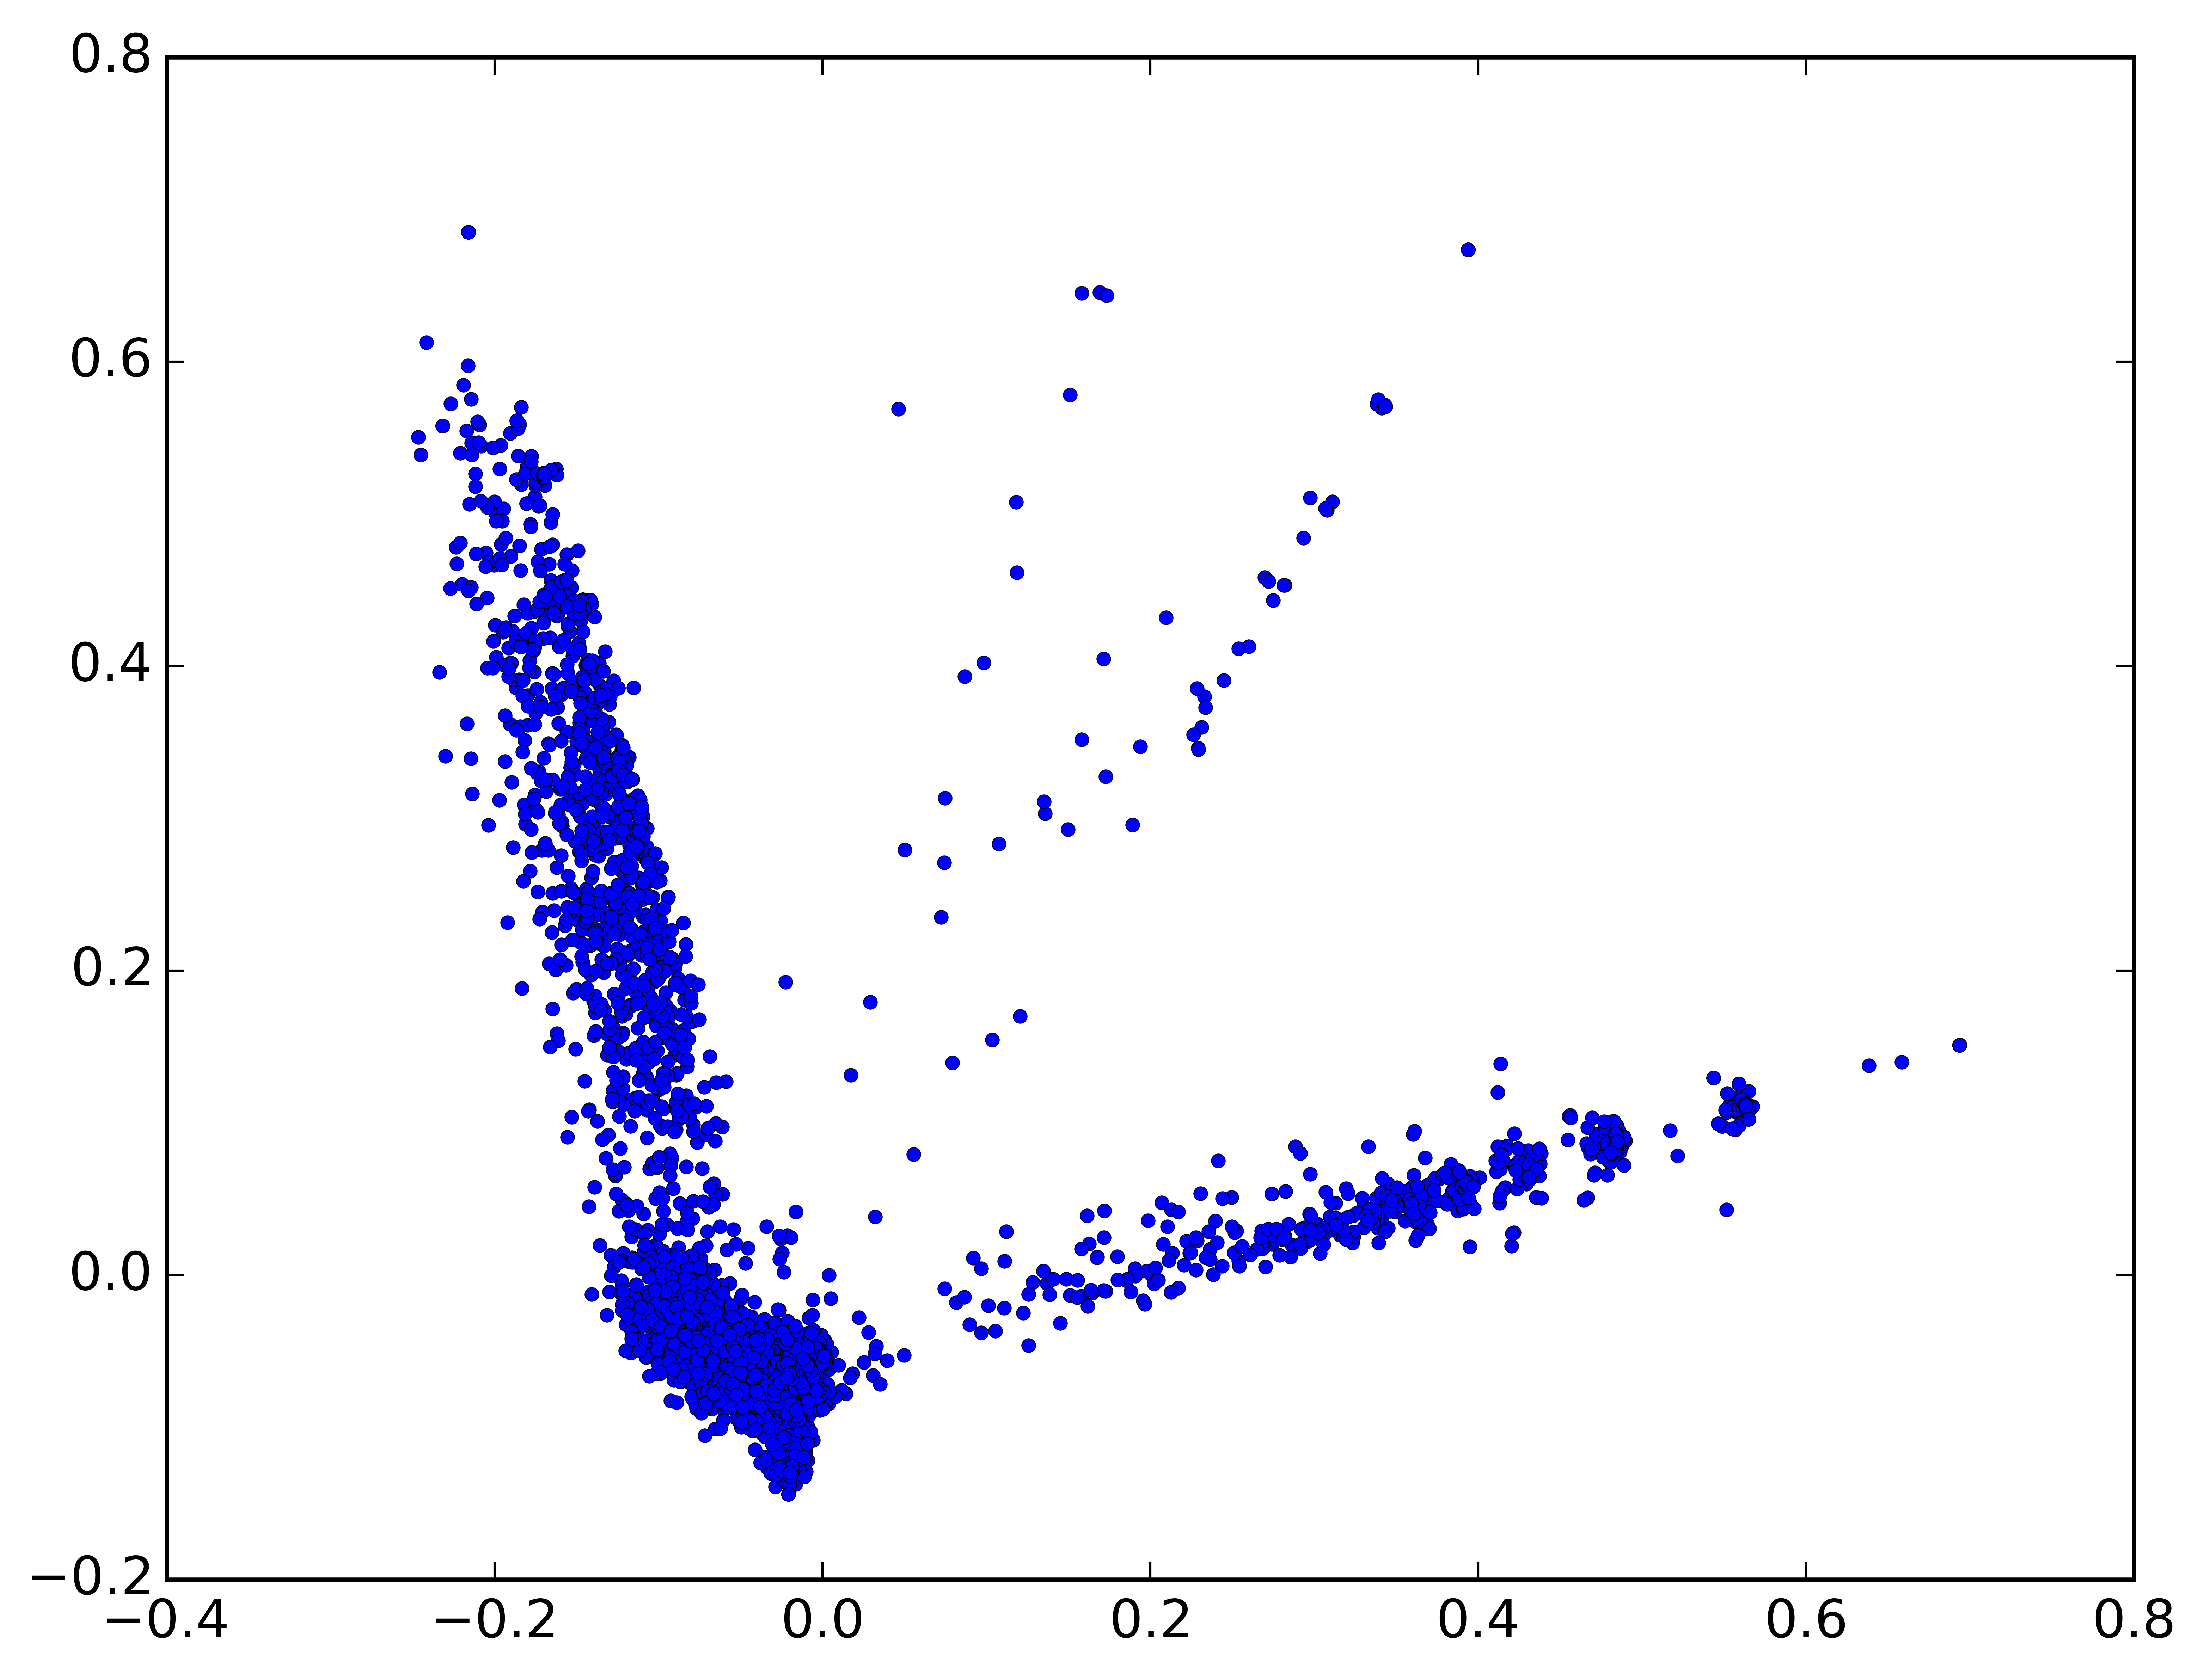
\includegraphics[width=\linewidth]{../images/mds_2d.png}
    \caption{2 Dimensions} \label{fig:mds:2d}
  \end{subfigure}
  \begin{subfigure}[t]{.49\linewidth}
    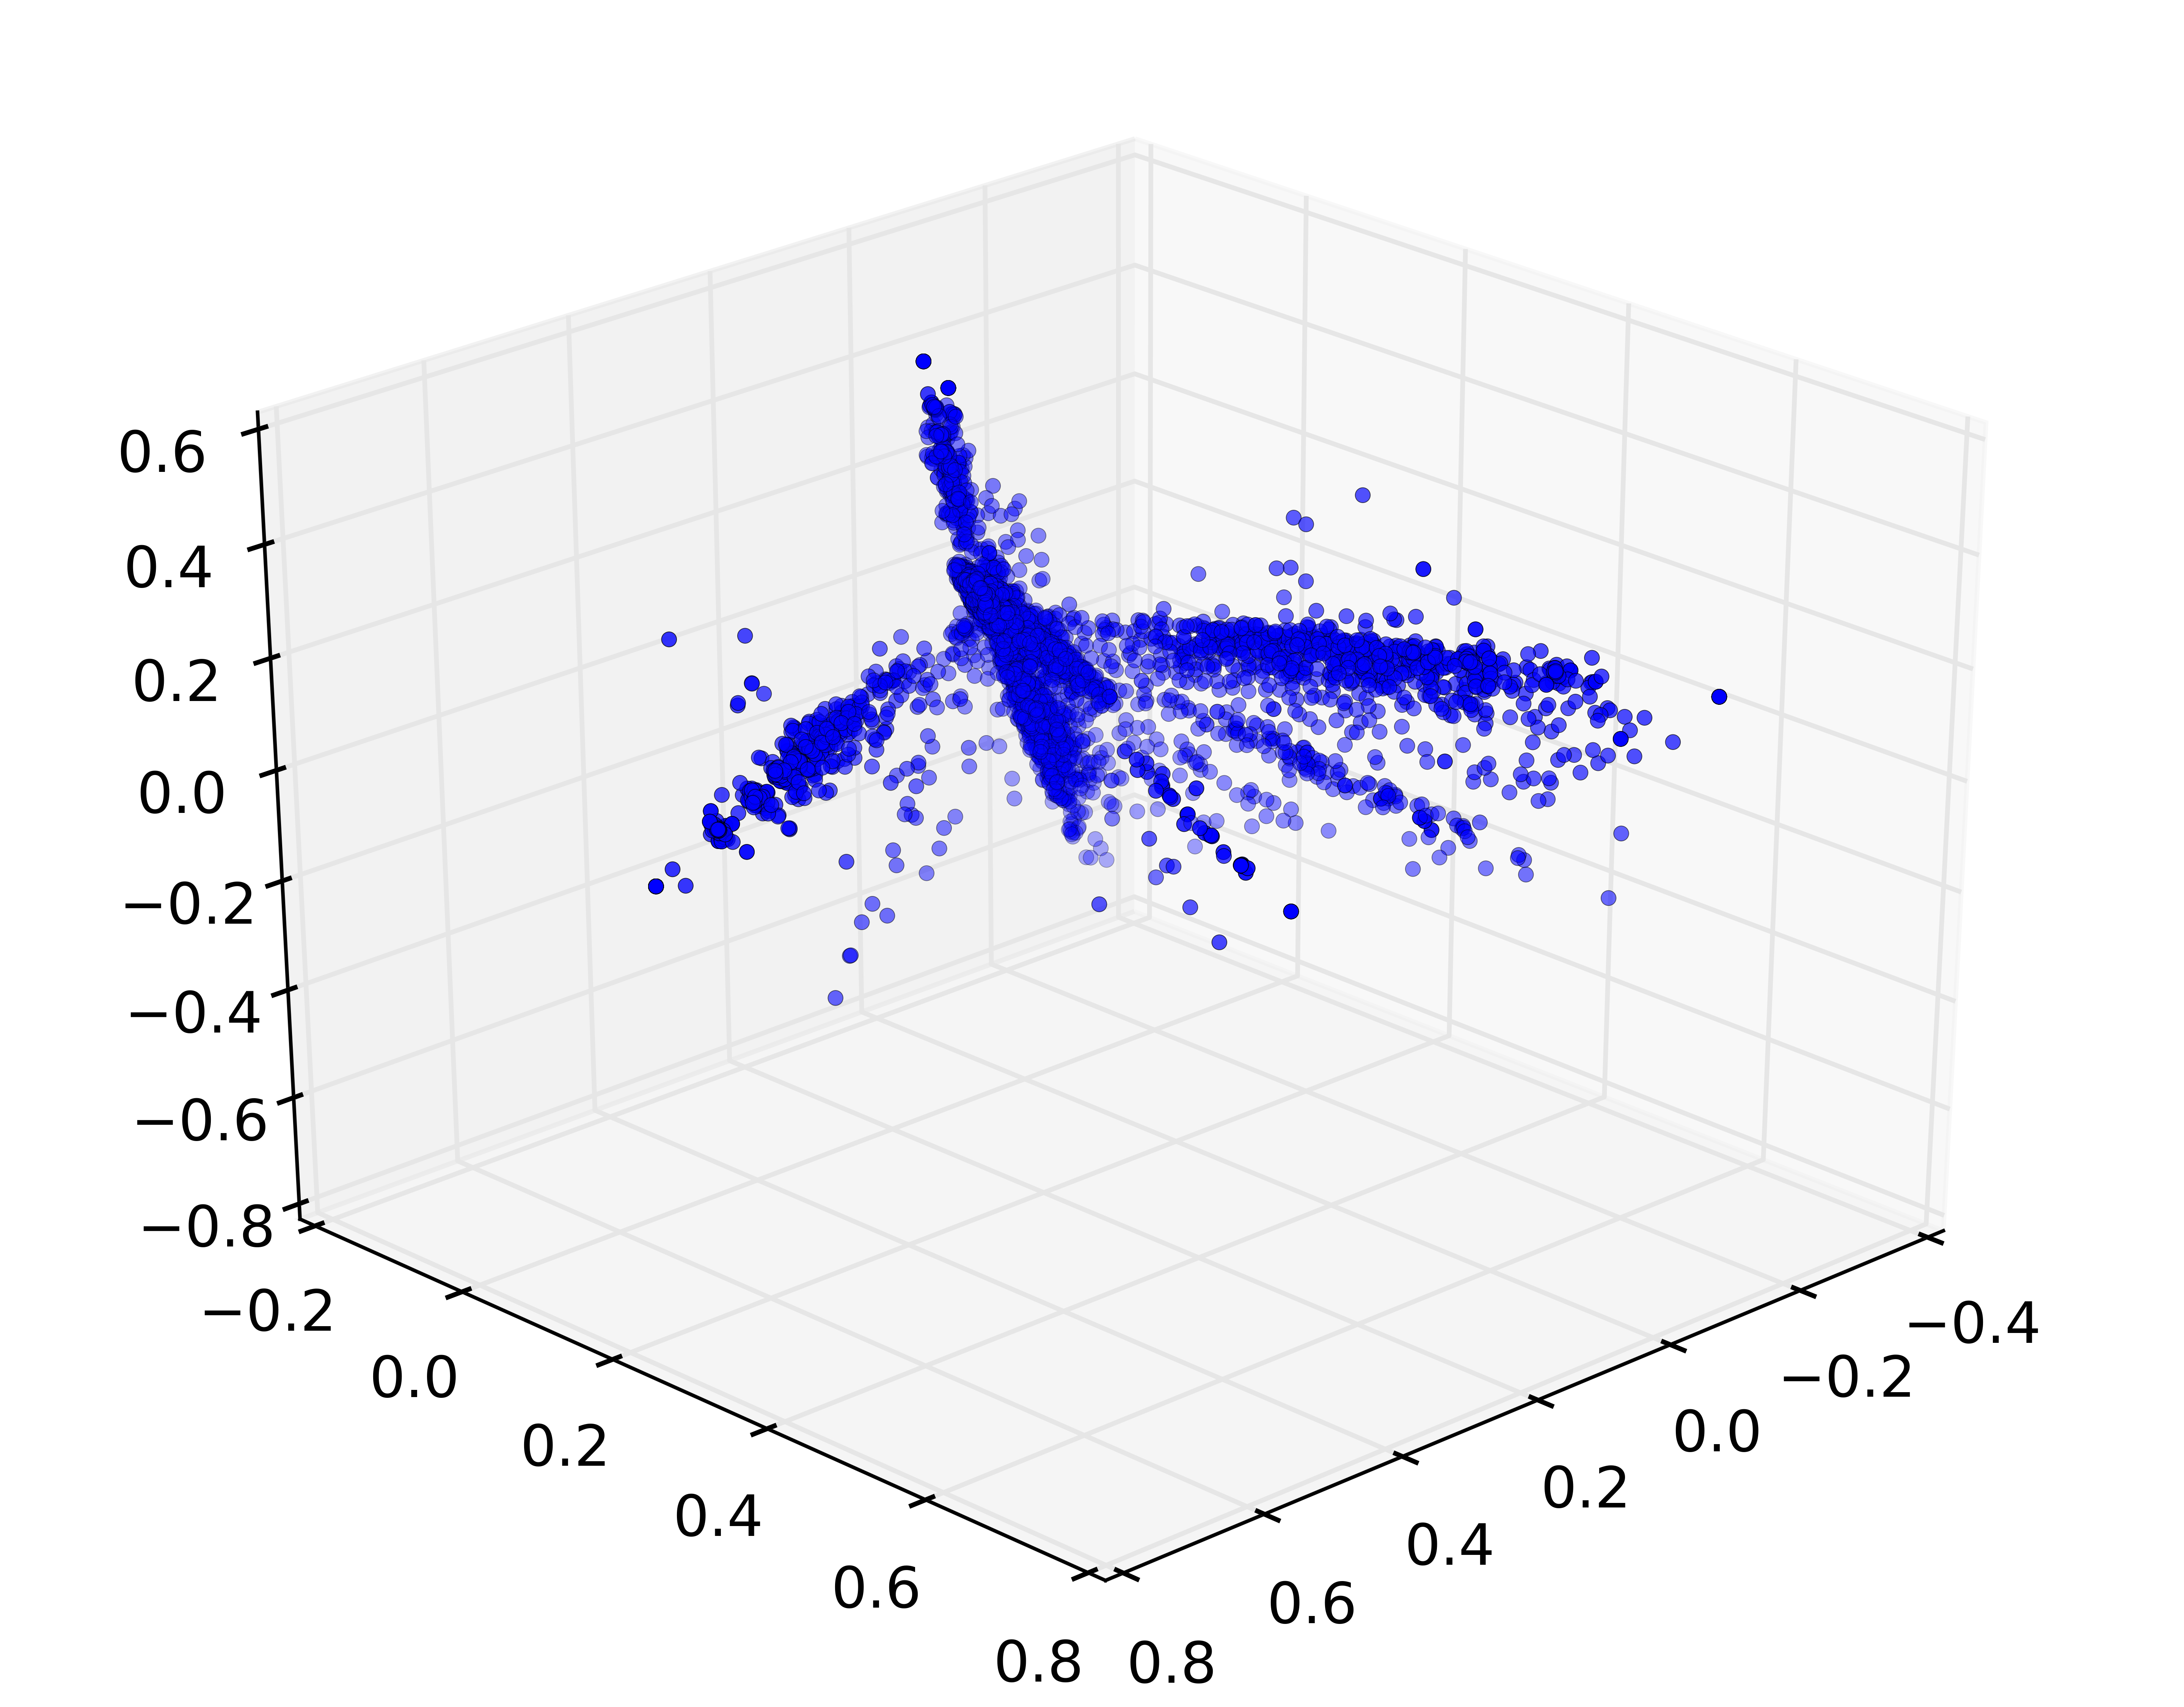
\includegraphics[width=\linewidth]{../images/mds_3d_1.png}
    \caption{3 Dimensions} \label{fig:mds:3d}
  \end{subfigure}
  \caption{Visualization of a 8,000 email subset using classical multi-dimensional scaling. The distance metric used is cosine distance as defined in Equation~\ref{eq:cos_dist}.}
  \label{fig:mds}
\end{figure}

\begin{figure}[htbp] \centering
  \begin{subfigure}[t]{.7\linewidth}
    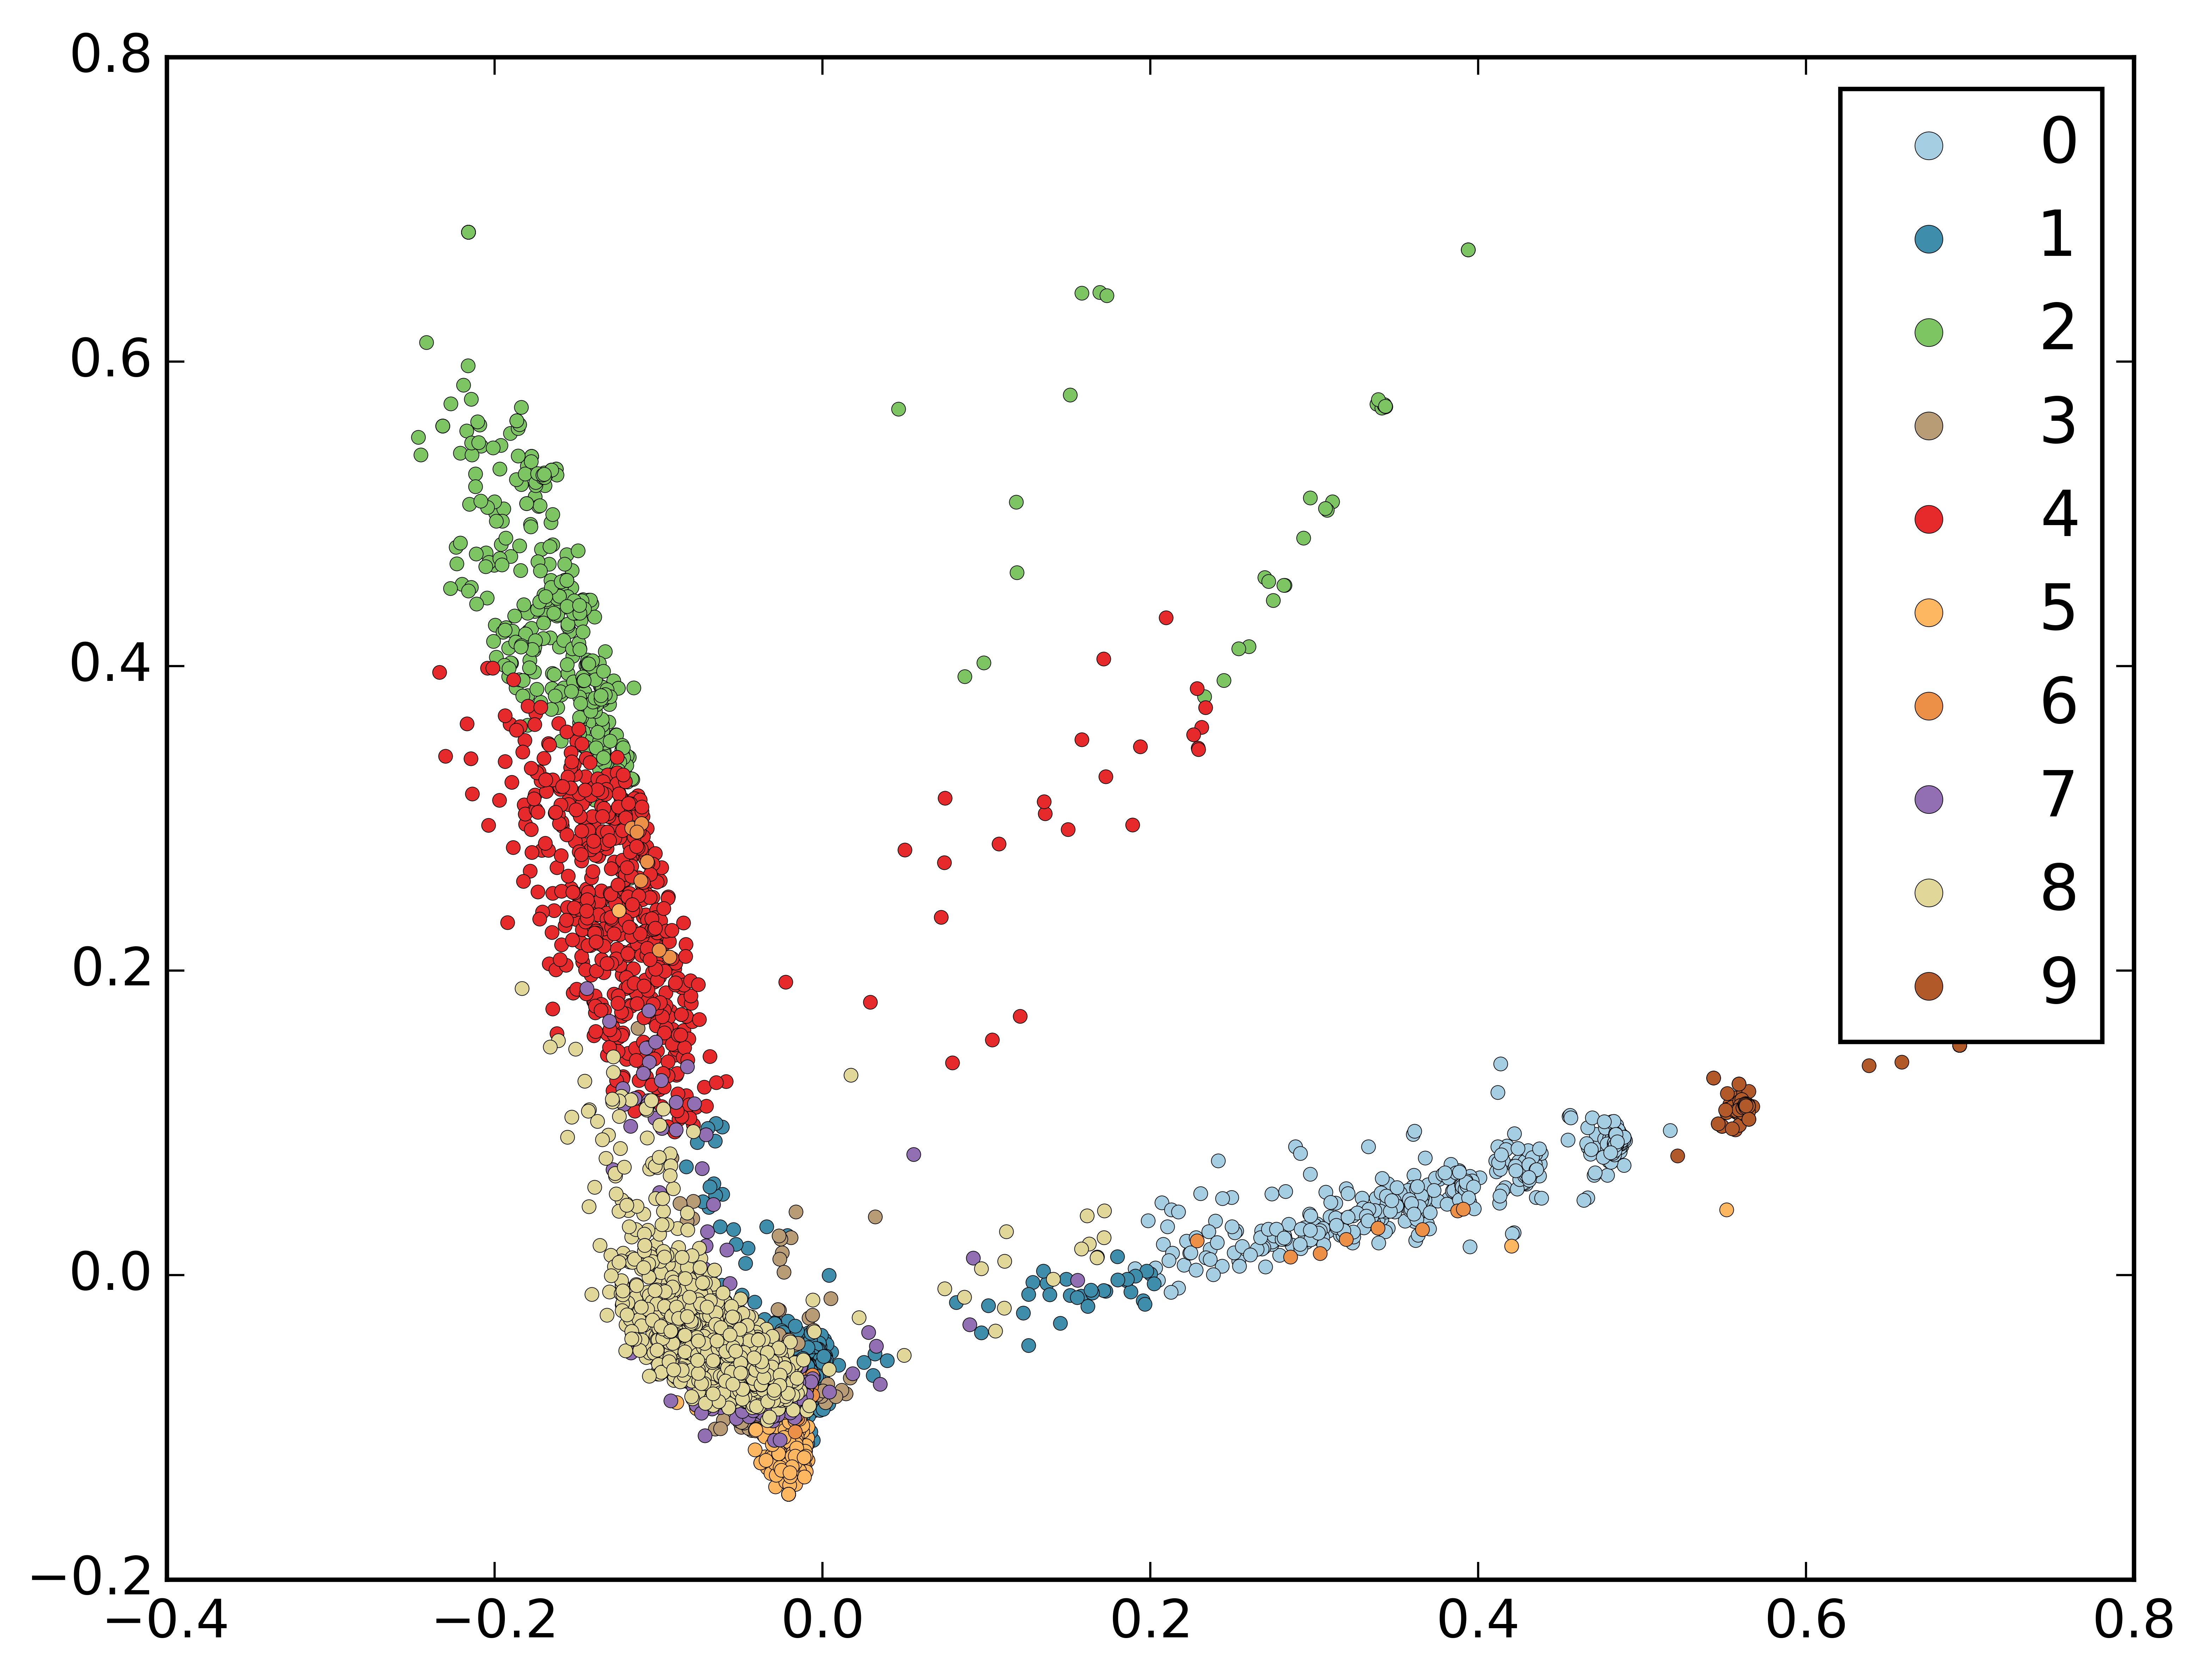
\includegraphics[width=\linewidth]{../images/mds_2d_cluster.png}
    \caption{2 Dimensions} \label{fig:cluster:2d}
  \end{subfigure}
  \begin{subfigure}[t]{.7\linewidth}
    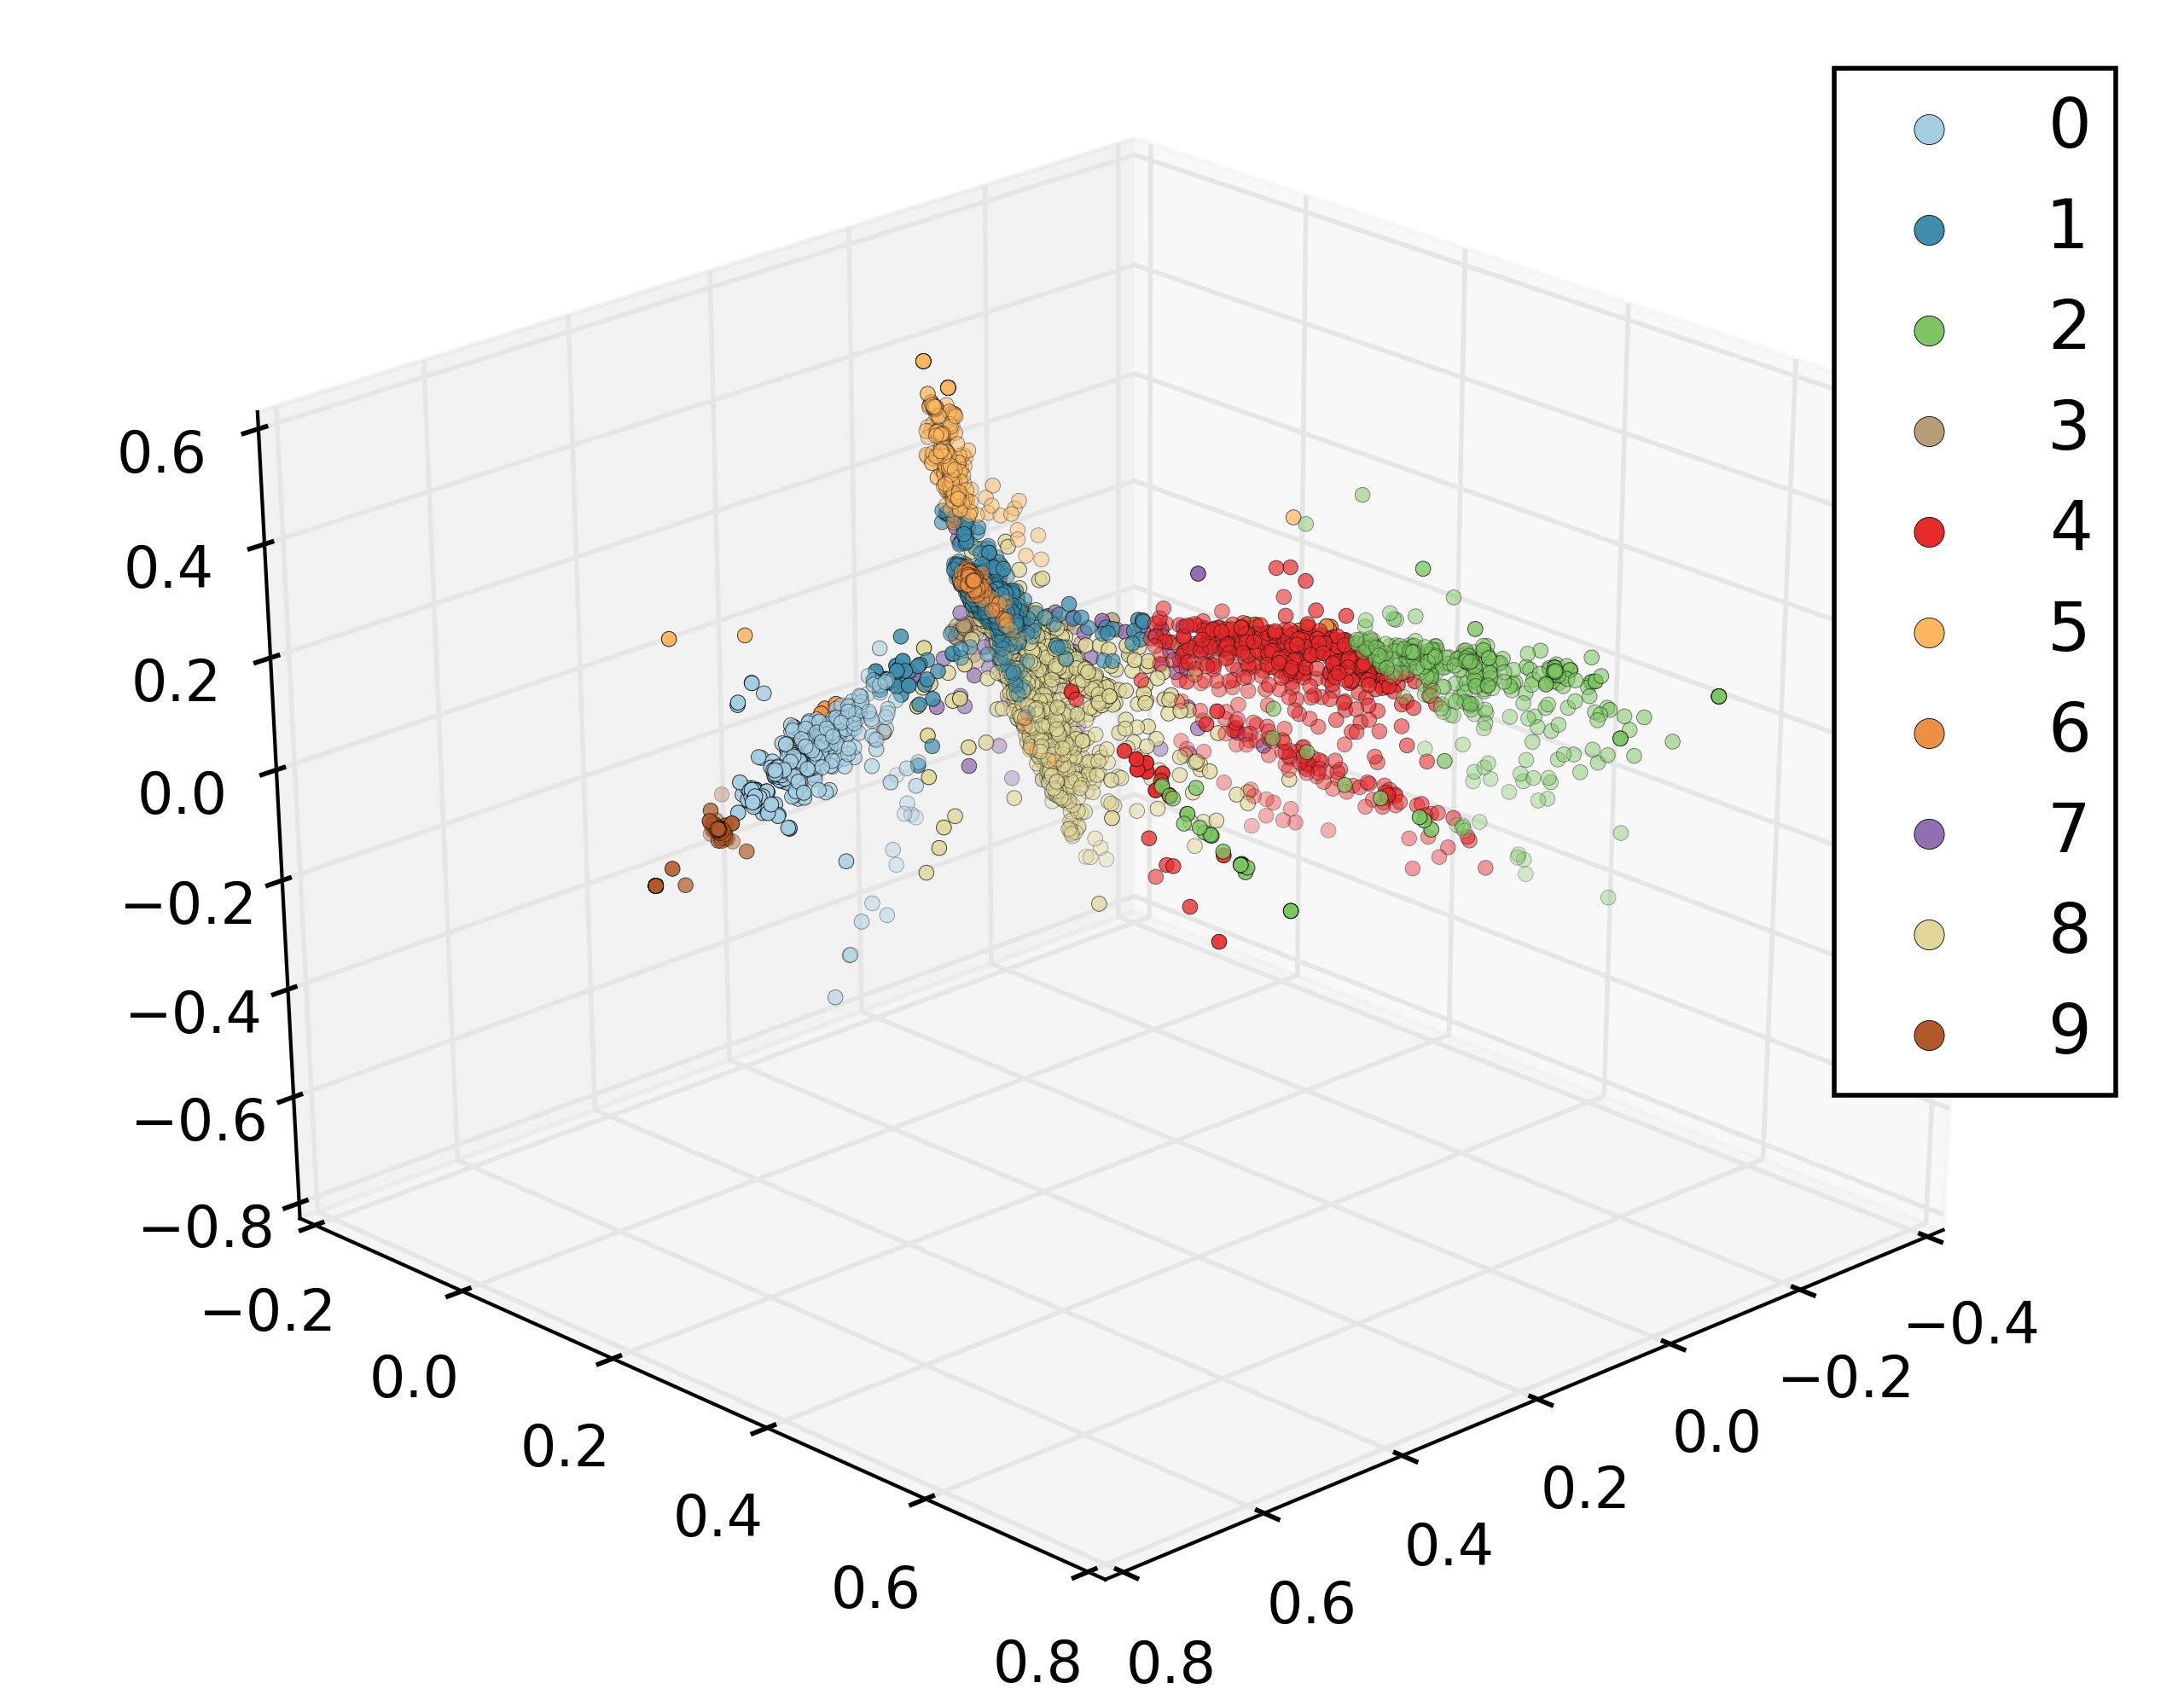
\includegraphics[width=\linewidth]{../images/mds_3d_cluster_1.png}
    \caption{3 Dimensions} \label{fig:cluster:3d}
  \end{subfigure}
  \caption{Visualization of the same 8,000 email subset with coloring according to the results from spectral clustering.}
  \label{fig:cluster}
\end{figure}


\subsection{Multidimensional Scaling}

\subsection{Spectral Clustering}


\section{Topic Modeling}
Include model description, estimation strategy, and model selection.

\subsection{Interpreting Topics}
Include ``grunt work'' of interpreting topics, topic frequency

\begin{table}[htb] \centering
\begin{tabular}{rcl}
  \toprule
  \colsquare{cterror}{10pt} & Terrorism & 5, 22 \\
  \colsquare{cmideast}{10pt} & Middle East & 6, 18, 19, 27, 29 \\
  \colsquare{cforeign}{10pt} & Foreign Policy & 2, 7, 13, 21, 23, 26 \\
  \colsquare{cpolitics}{10pt} & Politics & 11, 17, 25 \\
  \colsquare{cstaff}{10pt} & Staff & 16, 20 \\
  \colsquare{cpress}{10pt} & Press & 4 \\
  \colsquare{chill}{10pt} & Hillary & 12 \\
  \colsquare{cmeet}{10pt} & Meetings & 1, 9, 10, 24, 28, 30 \\
  \colsquare{ccomm}{10pt} & Common & 3, 8, 14, 15 \\
  \bottomrule
\end{tabular}
\caption{Topic Categorization}
\label{tab:topic_cat}
\end{table}

\begin{table}[htb] \centering
\setlength{\tabcolsep}{1pt}
\begin{tabular}{cccccccccccccccccccccccccc}
  \toprule
  \colsquare[-3pt]{cforeign}{16pt} &
  \colsquare[-3pt]{cmeet}{16pt} &
  \colsquare[-3pt]{cmeet}{16pt} &
  \colsquare[-3pt]{cmeet}{16pt} &
  \colsquare[-3pt]{cmeet}{16pt} &
  \colsquare[-3pt]{cmeet}{16pt} &
  \colsquare[-3pt]{cpress}{16pt} &
  \colsquare[-3pt]{cmeet}{16pt} &
  \colsquare[-3pt]{cmideast}{16pt} &
  \colsquare[-3pt]{cmideast}{16pt} &
  \colsquare[-3pt]{cstaff}{16pt} &
  \colsquare[-3pt]{chill}{16pt} &
  \colsquare[-3pt]{cstaff}{16pt} &
  \colsquare[-3pt]{cpolitics}{16pt} &
  \colsquare[-3pt]{cforeign}{16pt} &
  \colsquare[-3pt]{cmideast}{16pt} &
  \colsquare[-3pt]{cforeign}{16pt} &
  \colsquare[-3pt]{cmideast}{16pt} &
  \colsquare[-3pt]{cterror}{16pt} &
  \colsquare[-3pt]{cmideast}{16pt} &
  \colsquare[-3pt]{cforeign}{16pt} &
  \colsquare[-3pt]{cpolitics}{16pt} &
  \colsquare[-3pt]{cforeign}{16pt} &
  \colsquare[-3pt]{cforeign}{16pt} &
  \colsquare[-3pt]{cpolitics}{16pt} &
  \colsquare[-3pt]{cterror}{16pt} \\
  21 & 1 & 28 & 30 & 10 & 9 & 4 & 24 & 18 & 29 & 16 & 12 & 20 &
  17 & 13 & 19 & 23 & 27 & 22 & 6 & 2 & 25 & 26 & 7 & 11 & 5 \\
  \midrule
  \multicolumn{13}{l}{Most Frequent} & \multicolumn{13}{r}{Least Frequent} \\
  \bottomrule
\end{tabular}
\setlength{\tabcolsep}{6pt}
\caption{Primary Topic Frequency}
\label{tab:topic_freq}
\end{table}


\subsection{Types of Topics}
Talk about structural, common word, and semantic topics, including ``interesting'' vs. ``non-interesting'' topics, discuss strengths of model in comparison to MDS

\subsection{Topic Analysis}
Analyze some specific topics, compare use over time and how it correlates with related events


\section{Email Sender Prediction}
Talk about the who says what table

\subsection{Multinomial Logistic Regression}
Quickly describe model and discuss results


\section{Conclusion}



\end{document}
